\graphicspath{{experimental_setup/fig/}}

\chapter{Experimental Setup} \label{chap:experimental_setup}
This chapter provides our research questions, and how we attempt to answer
these questions using the results of different experiments. We discuss the datasets used for
our ASR models, as well as the data for our language model (LM).
The chapter concludes with a discussion of the metrics used in this study to evaluate our ASR models.

\section{Research questions and experiments}
The main research question we attempt to answer in this study is: ``Does a sequential fine-tuning strategy, where the model is first fine-tuned on (for example) Afrikaans data and subsequently on isiXhosa data, result in better accuracy and generalization performance compared to fine-tuning on isiXhosa data alone?''.
We investigate this research question by fine-tuning Wav2Vec2-Large and XLS-R using:
\begin{enumerate}
    \item Only Afrikaans data.
    \item Only isiXhosa data.
    \item isiXhosa data, and then Afrikaans data.
    \item Afrikaans data, and then isiXhosa data.
\end{enumerate}
Experiments (1) and (3), and experiments (2) and (4) are compared using WER (\ref{subsec:wer}).
Additionally, each model is also evaluated with and without the use of a $5$-gram LM with Kneser-Ney smoothing \cite{shannon1948}, \cite{ney1994structuring}.

\section{Data sets}
We use three different data sources to create an \href{https://huggingface.co/datasets/lucas-meyer/asr_af}{Afrikaans dataset} and an \href{https://huggingface.co/datasets/lucas-meyer/asr_xh}{isiXhosa dataset}, which contains labeled speech recordings.
The three data sources are briefly explained in the paragraphs below.

\paragraph*{NCHLT dataset.}
The NCHLT \cite{barnard2014nchlt} dataset contains speech recordings for the eleven official South African languages.
The dataset contains approximately $200$ speakers per language.
The NCHLT recordings (on average) are the shortest of the three datasets, with most recordings being between $2$ and $6$ seconds.
Based on brief inspection, the transcription texts of this dataset contain very few words, and rarely contain full sentences.

\paragraph*{FLEURS dataset.}
The FLEURS \cite{fleurs2022arxiv} dataset contains speech recordings for $102$ different languages, including Afrikaans, isiXhosa, and isiZulu.
Each language has its own training, validation, and test set split.
No information is given about the number of speakers for each language.
The FLEURS recordings (on average) are the longest of the three datasets, with most recordings being between $7$ and $20$ seconds.
Based on brief inspection, the transcription texts of this dataset contain full sentences.

\paragraph*{High-quality TTS dataset.}
The High-quality text-to-speech (TTSs) \cite{hq2017} dataset contains high quality transcribed audio data for four South African languages: Afrikaans, Sesotho, Setswana and isiXhosa.
There are nine Afrikaans speakers and 12 isiXhosa speakers.
The duration of most recordings are between $5$ and $10$ seconds.
Based on brief inspection, the transcription texts of this dataset contain mostly full sentences, and a few that contain short phrases.
\\
\\
We select the recordings for the Afrikaans and isiXhosa dataset to have similar distributions for the durations of the recordings.
Figure \ref{fig:histogram} describes the duration histograms of the two datasets. Despite the large number of short recordings, we omit
most of the NCHLT dataset, in favor of longer recordings with full sentence transcription texts.

\begin{figure}[!ht]
    \centering
    \captionsetup{justification=centering}
    \begin{minipage}{.5\textwidth}
      \centering
      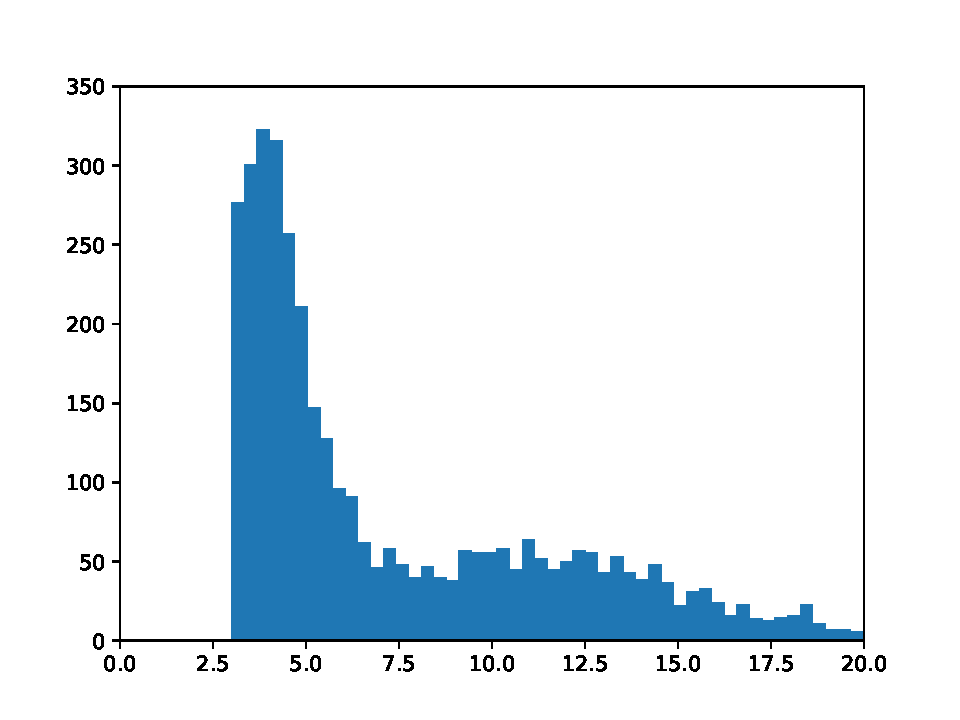
\includegraphics[width=\linewidth]{final_histogram_af.pdf}
    \end{minipage}%
    \begin{minipage}{.5\textwidth}
      \centering
      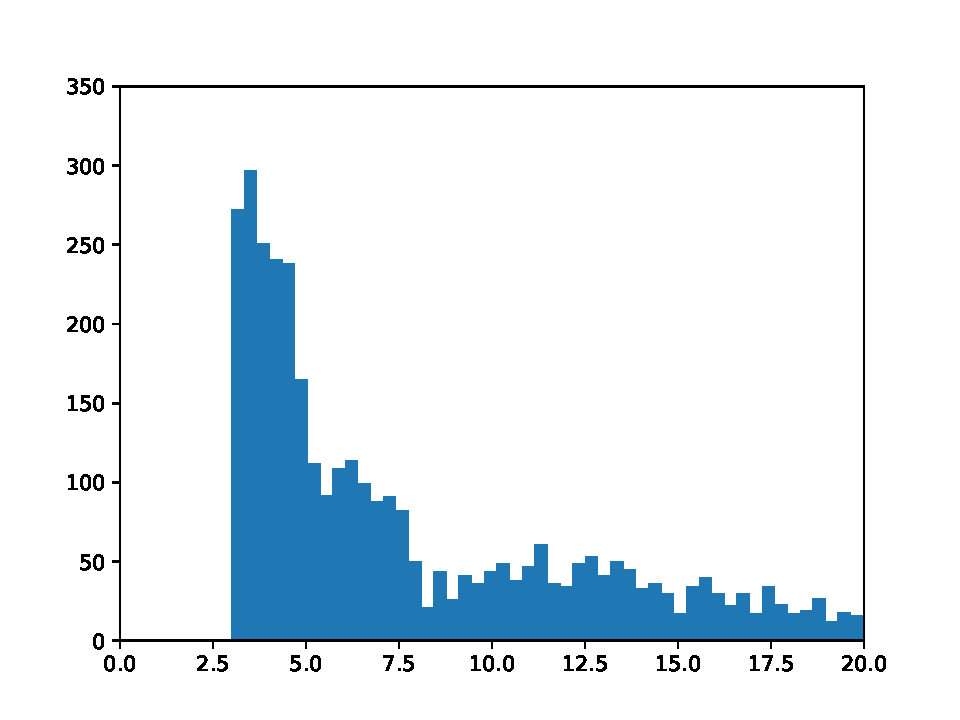
\includegraphics[width=\linewidth]{final_histogram_xh.pdf}
    \end{minipage}
    \caption{The histograms of the recording durations of the Afrikaans dataset (left) and the isiXhosa dataset (right)}
    \label{fig:histogram}
\end{figure}

We ensure that the validation and test set splits do not contain recordings of speakers that appear in the training set split.
Both of the datasets contain approximately $7.5$ hours of speech recordings.
All of the speech recordings are downsampled to a sample rate of $16,000$ Hz, which is the expected sample rate of Wav2Vec2-Large and XLS-R.
The transcription texts are pre-processed in the same way as the LM data, which is explained in the following section.

\subsection{Language model data}
The data used for training the LM (\ref{subsec:lm-boost}) consists of \href{https://dumps.wikimedia.org/}{Wikipedia dumps}.
The text is extracted from the dumps using a tool called the WikiExtractor \cite{Wikiextractor2015}.
The text is pre-processed by converting all characters to lowercase, removing all characters that are not used in the Afrikaans
and isiXhosa language, and removing punctuation marks and other special characters.

\section{Evaluation metrics}

\paragraph*{Word error rate} \label{subsec:wer}
The word error rate (WER) is equal to the number of character-level errors in the predicted transcript, 
divided by the number of words in the true transcript. One character-level error is corrected using one of three operations:
inserting a new character, deleting an existing character, or substituting an existing character for a new character.
